The human brain is composed of billions of neurons, interconnected electrically excitable cells that form the basis of intelligence.
Each neuron has dendrites that receive electrical signals from other neurons.
If the sum of these electrical signals is greater than a certain threshold value, the neuron fires, propagating a voltage down its axon and out of its synapses.
These synapses can be considered the output of the neuron and are themselves connected to the dendrites of other neurons.
The interconnections of these neurons form a massive network, where a huge number of inputs are processed in parallel to a set of outputs.
The purpose of artificial neural networks is to simulate the mathematical properties of these neurons in order to approximate complex functions.

\subsection{Single Artificial Neuron}

\begin{figure}[ht]
	\centering
	\def\layersep{2.5cm}
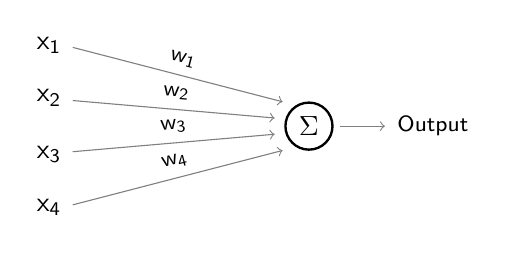
\begin{tikzpicture}[font=\sffamily,shorten >=1pt,->,draw=black!50, node distance=\layersep]
    \tikzstyle{every pin edge}=[<-,shorten <=1pt]
    \tikzstyle{neuron}=[circle,line width=0.3mm,draw=black,minimum size=17pt,inner sep=0pt]
    \tikzstyle{annot} = [text width=4em, text centered]


    \draw[->] (-3,1) -- (-.3,.3) node[sloped,midway,above] {\footnotesize w\textsubscript{1}} node[left=3cm,above=.5cm]{x\textsubscript{1}};

    \draw[->] (-3,0.325) -- (-.4,.1) node[sloped,midway,above] {\footnotesize w\textsubscript{2}} node[left=2.9cm,above=.03cm]{x\textsubscript{2}};
 
    \draw[->] (-3,-.325) -- (-.4,-.1) node[sloped,midway,above] {\footnotesize w\textsubscript{3}} node[left=2.9cm,below=.03cm]{x\textsubscript{3}};
 
    \draw[->] (-3,-1) -- (-.3,-.3) node[sloped,midway,above] {\footnotesize w\textsubscript{4}} node[left=3cm,below=.5cm]{x\textsubscript{4}};
    
    \node[neuron] (0,0) {$\Sigma$};

    \draw[->] (.4,0) -- (1,0) node[right] {\footnotesize Output};
\end{tikzpicture}
	\caption{Single Neuron Diagram}
\end{figure}

An artificial neuron is simply a mathematical model of a biological neuron, and therefore its functionality is very similar.
Each artificial neuron has multiple inputs.
In addition, each neuron has a weight for each input, a bias term, an activation function, and one output.
The output of one neuron becomes the input of other connected neurons.
The output of a neuron is expressed mathematically for $n$ inputs $x$ and weights $w$, a bias term $b$, and activation function $O(x)$:

\begin{align*}
	\text{activation} = \sum_{i=0}^{n}x_i w_i + b\\
	\text{output} = O(\text{activation})
	\,.
\end{align*}

A weight is a positive or negative number that governs the impact of of its respective input on the neuron's single output.
The activation function transforms the output of the neural network. Common activation functions include a sigmoid curve, a hyperbolic tangent, a binary step function, and a rectifier function. Fido uses the sigmoid activation function since it is gradient, has a fixed range, and is easily differentiable.
The bias term is a number added to the summation of weights and inputs, allowing us to make affine transformations on the domain of the activation function.

\begin{figure}[ht]
	\centering
	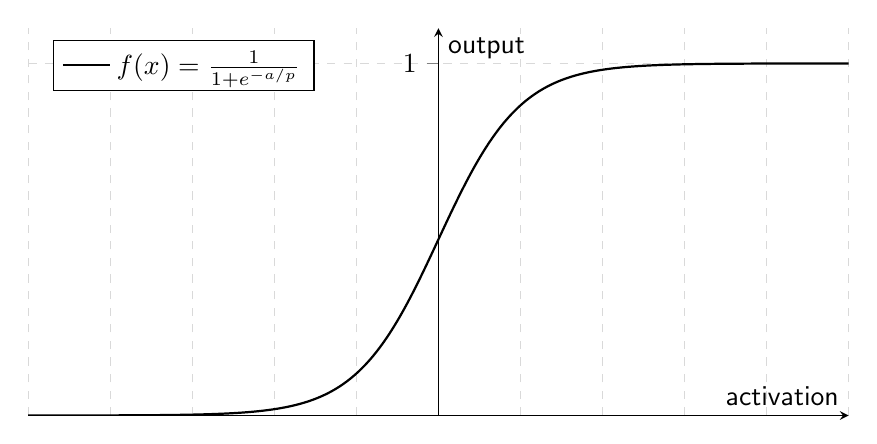
\begin{tikzpicture}[font=\sffamily]
    \begin{axis}[
    	legend pos=north west,
        axis x line=middle,
        axis y line=middle,
        grid = major,
        width=12cm,
        height=6.5cm,
        grid style={dashed, gray!30},
        xmin=-1,xmax= 1,ymin= 0,ymax= 1.1,
        xlabel=activation,ylabel=output,
        tick align=outside,
        ytick={1},
        xmajorticks=false,
        enlargelimits=false]
      \addplot[domain=-1:1,black,thick,samples=500] {1/(1+exp(-10*x))}; 
      \addlegendentry{$f(x)=\frac{1}{1+e^{-a/p}}$}
    \end{axis} 
\end{tikzpicture}
	\caption{Sigmoid Activation Function Graph}
\end{figure}

\subsection{Feed-forward Neural Network}

Fido utilizes a feed-forward neural network, a collection of neurons organized into layers, as a function appropriator in its machine learning algorithm. In a feed-forward neural network, the output of each neuron is the input of each neuron in the next layer.
In this way, the original inputs of the neural network are ``fed forward'' layer by layer, starting from the first layer (the input layer), passing through any number of middle layers (hidden layers), and ending with the last layer (the output layer).
The outputs of the neurons in the output layer are the outputs of the whole network.

\begin{figure}[ht]
	\centering
	\def\layersep{2.5cm}
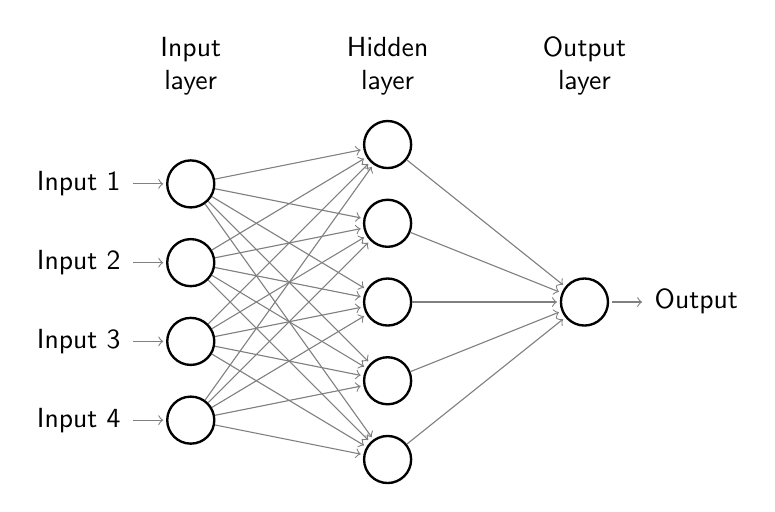
\begin{tikzpicture}[shorten >=1pt,->,draw=black!50, node distance=\layersep,font=\sffamily]
    \tikzstyle{every pin edge}=[<-,shorten <=1pt]
    \tikzstyle{neuron}=[circle,line width=0.3mm,draw=black,minimum size=17pt,inner sep=0pt]
    \tikzstyle{annot} = [text width=4em, text centered]

    \foreach \name / \y in {1,...,4}
        \node[neuron, pin=left:Input \y] (I-\name) at (0,-\y) {};

    \foreach \name / \y in {1,...,5}
        \path[yshift=0.5cm]
            node[neuron] (H-\name) at (\layersep,-\y cm) {};

    \node[neuron,pin={[pin edge={->}]right:Output}, right of=H-3] (O) {};

    \foreach \source in {1,...,4}
        \foreach \dest in {1,...,5}
            \path (I-\source) edge (H-\dest);

    \foreach \source in {1,...,5}
        \path (H-\source) edge (O);

    %\draw[->] (5,-2.9) -- (5,-5) -- (1,-5) -- (1,-4.5);
    %\node (1,-4.5) {Error back propagation}

    \node[annot,above of=H-1, node distance=1cm] (hl) {Hidden layer};
    \node[annot,left of=hl] {Input layer};
    \node[annot,right of=hl] {Output layer};
\end{tikzpicture}
	\caption{A Feed-forward Neural Network}
	\label{fig:feedforward}
\end{figure}

\subsection{Backpropagation}

Supervised learning is the modification of the weights of a neural network's neurons in order to reach a specific output from a specific set of inputs.
One such method of adjusting neural networks weights is called back propagation \cite{werbos}.

\begin{figure}[ht]
	\centering
	\def\layersep{2.5cm}
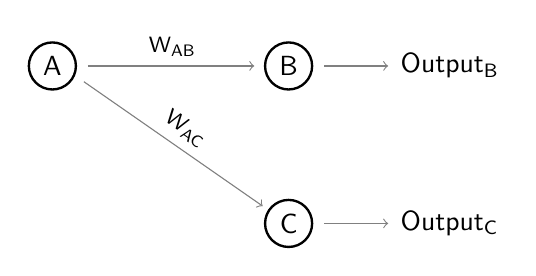
\begin{tikzpicture}[font=\sffamily,shorten >=1pt,->,draw=black!50, node distance=\layersep]
    \tikzstyle{every pin edge}=[<-,shorten <=1pt]
    \tikzstyle{neuron}=[circle,line width=0.3mm,draw=black,minimum size=17pt,inner sep=0pt]
    \tikzstyle{annot} = [text width=4em, text centered]

    \draw[->] (.45,0) -- (2.6,0) node[sloped,midway,above] {\footnotesize W\textsubscript{AB}};
    \draw[->] (.4,-.2) -- (2.7,-1.8) node[sloped,midway,above] {\footnotesize W\textsubscript{AC}};

    \draw[->] (3.45,0) -- (4.3,0) node[right=0cm]{Output\textsubscript{B}};
    \draw[->] (3.45,-2) -- (4.3,-2) node[right=0cm]{Output\textsubscript{C}};
    
    \node[neuron] at (0,0) {A};
    \node[neuron] at (3,0) {B};
    \node[neuron] at (3,-2) {C};
\end{tikzpicture}
	\caption{Single Branch in a Back Propagation Neural Network}
	\label{fig:backprop}
\end{figure}

Neural networks learning through back propagation are trained through example.
Example inputs (known as training sets) are linked to a particular target output, forming a training pair.
The first step of training is to pass in an arbitrary training set to a neural network with randomly generated weights.
The error $\delta$ for an output neuron is defined as the difference between the actual output and the target output for that training set.
As an example we will use the single connection described in Figure \ref{fig:backprop}.
The neural network in this figure has only an input layer consisting of Neuron $A$ and an output layer consisting of Neurons $A$ and $B$.
$W_{AB}$  and $W_{AC}$ are the weights between the neurons.
We first determine the Neuron $B$ error $\delta_B$ as $\text{Target}_B - \text{Output}_B$.
 Next we modify weight $W_{AB}$ as follows, defining $W_{AB}^{+}$ as the newly trained weight:

\begin{equation}
	W_{AB}^{+} = W_{AB} + (\delta_B \text{Output}_A)\,.
\end{equation}

The same approach could be taken for Neuron $C$.
However, this method cannot calculate an improved weight for hidden layer neurons such as Neuron $A$, as there is no predefined target.
Therefore we must calculate the error of $A$ indirectly by back propagating from the two output layer neurons, for which the error is already known:

\begin{equation}
	\delta_A = W_{AB}\delta_B + W_{AC}\delta_C \,.
\end{equation}

Once the error for Neuron $A$ is obtained, its trained weights can be calculated in the same fashion as done for Neuron $B$.
This pattern can be repeated throughout a larger neural network in order to converge upon the network's target output.

\subsection{Q-Learning}

Fido is a reinforcement learning system. Reinforcement learning systems seek to find the optimal action to be undertaken for a given state through trial and error.
In the context of Fido, an action could be the playing of a note or driving straight forwards, while the state could be the amount of light detected by the robot or how near the robot is to another object.
Once an action is performed, a reward and a new state are given back to the reinforcement learning algorithm.
As actions are performed over time, the reinforcement learning algorithm sharpens its ability to receive reward.

$Q$-Learning \cite{watkins} is a popular reinforcement learning algorithm that works by learning an action-value function $Q$ that takes a state-action pair as an input and outputs the expected utility value of performing that action in that state.
This utility value is know as the $Q$-value.
The $Q$-value is a combination of immediate reward and expected future reward.
Every learning iteration the $Q$-value of an state-action pair is updated as such:

\begin{equation}
	Q(s, a) := Q(s, a)(1 - \alpha) + \alpha(R + \gamma \max Q(s_{t+1}, a))
	\,,
	\label{equ::updateqlearn}
\end{equation}

\noindent
where $a$ is the action carried out, $s$ is the initial state, $R$ is the reward received, and $s_{t+1}$ is the new state.
$\alpha$ is the learning rate of the algorithm.
The learning rate determines the rate of convergence by diminishing or amplifying the changes made to the $Q$-value each learning iteration.
$\gamma$ is the devaluation factor, which determines the weight given to future rewards.
A devaluation factor approaching $\gamma=0$ will force the algorithm to only value immediate reward, while a devaluation factor approaching $\gamma=1$ will make it focused on high long term reward.

A table was originally used to model the $Q$ function, storing state-action pairs and each pair's respective $Q$-value.
However, in recent years, neural networks have been increasingly used to model the $Q$-function, since they can generalize between similar states, and so, converge in less time than a table based implementation.
For the purposes of this paper, the "industry standard" is discrete-action $Q$-learning coupled with feed-forward neural networks.
